\chapter{Parsing}

After Lexical Analysis is complete and the input string has been tokenised the next step is to generate a parse tree.  Parsers produce a data structure that takes into account all the details of the language defied in its grammar and also attempt to perform error handing.

\section{Building Parse Trees}

A parser takes the output from lexical analysis and turns it into a tree data structure.  This tree structure enforces properties not apparent from just a linear sequence of tokens such as associativity.  The structure also validates the input by checking it against the grammar for the language.  

One of the features of a user friendly parser is reporting errors that the user has made in the input to the application to assist in fixing the input.


\section{Parsing Blazon}

Parsing Blazon involves taking the tokens generated form Lexical analysis and producing a well formed data structure that checks whether the input conforms to the defied grammar or not and attempts to report the reason behind why the input may be erroneous.

Blazon lends it self very well to a top down, left to right parsing method because of the way the language is defined. Fields are defined and Tinctured from the top-left most point downwards and mirroring this approach in parsing makes for a nice parallel. 

The output from the lexical analysis is of a fairly high level because of the more advanced lexing approach taken which wrapped Line Types, Quantifiers and Tinctures into other objects when appropriate.  

To build the data structure itself each of the objects to be instantiated have inbuilt class variables to allows them to act as nodes in a tree. 

Partitions all have an array, the size of which is determined by the number of fields to be created for the particular type of partition.  Tinctures have an array of Charges so that they can have multiple charges placed upon them. 

As Blazon sentences all implicitly start with an empty field that encompass the entire shied this is where the parser and parse tree will start.  In the implementation the implicit field is represented by a partition which produces a single field,  an \emph{Escutcheon}. 

The parser then takes the first token, according to the grammar the only valid operations that can be performed upon a field are Tincturing it or Partitioning it, therefore the parser checks whether this token is either a Tincture or a Partition and if it either of the above adds it to the initial field accordingly.  

This process is repeated until either there are no more tokens left to parse, no more space in the tree structure exists, upon a valid Blazon sentence, both. 



\section{An Example of Parsing Blazon}


The following demonstrates the parsing of the Blazon sentence \emph{Per Bend Azure and Or a Cross Vert}.  

The tokens generated by Lexical analysis would be, \emph{Partition (Bend), }


\begin{figure}[H]
  \centering
    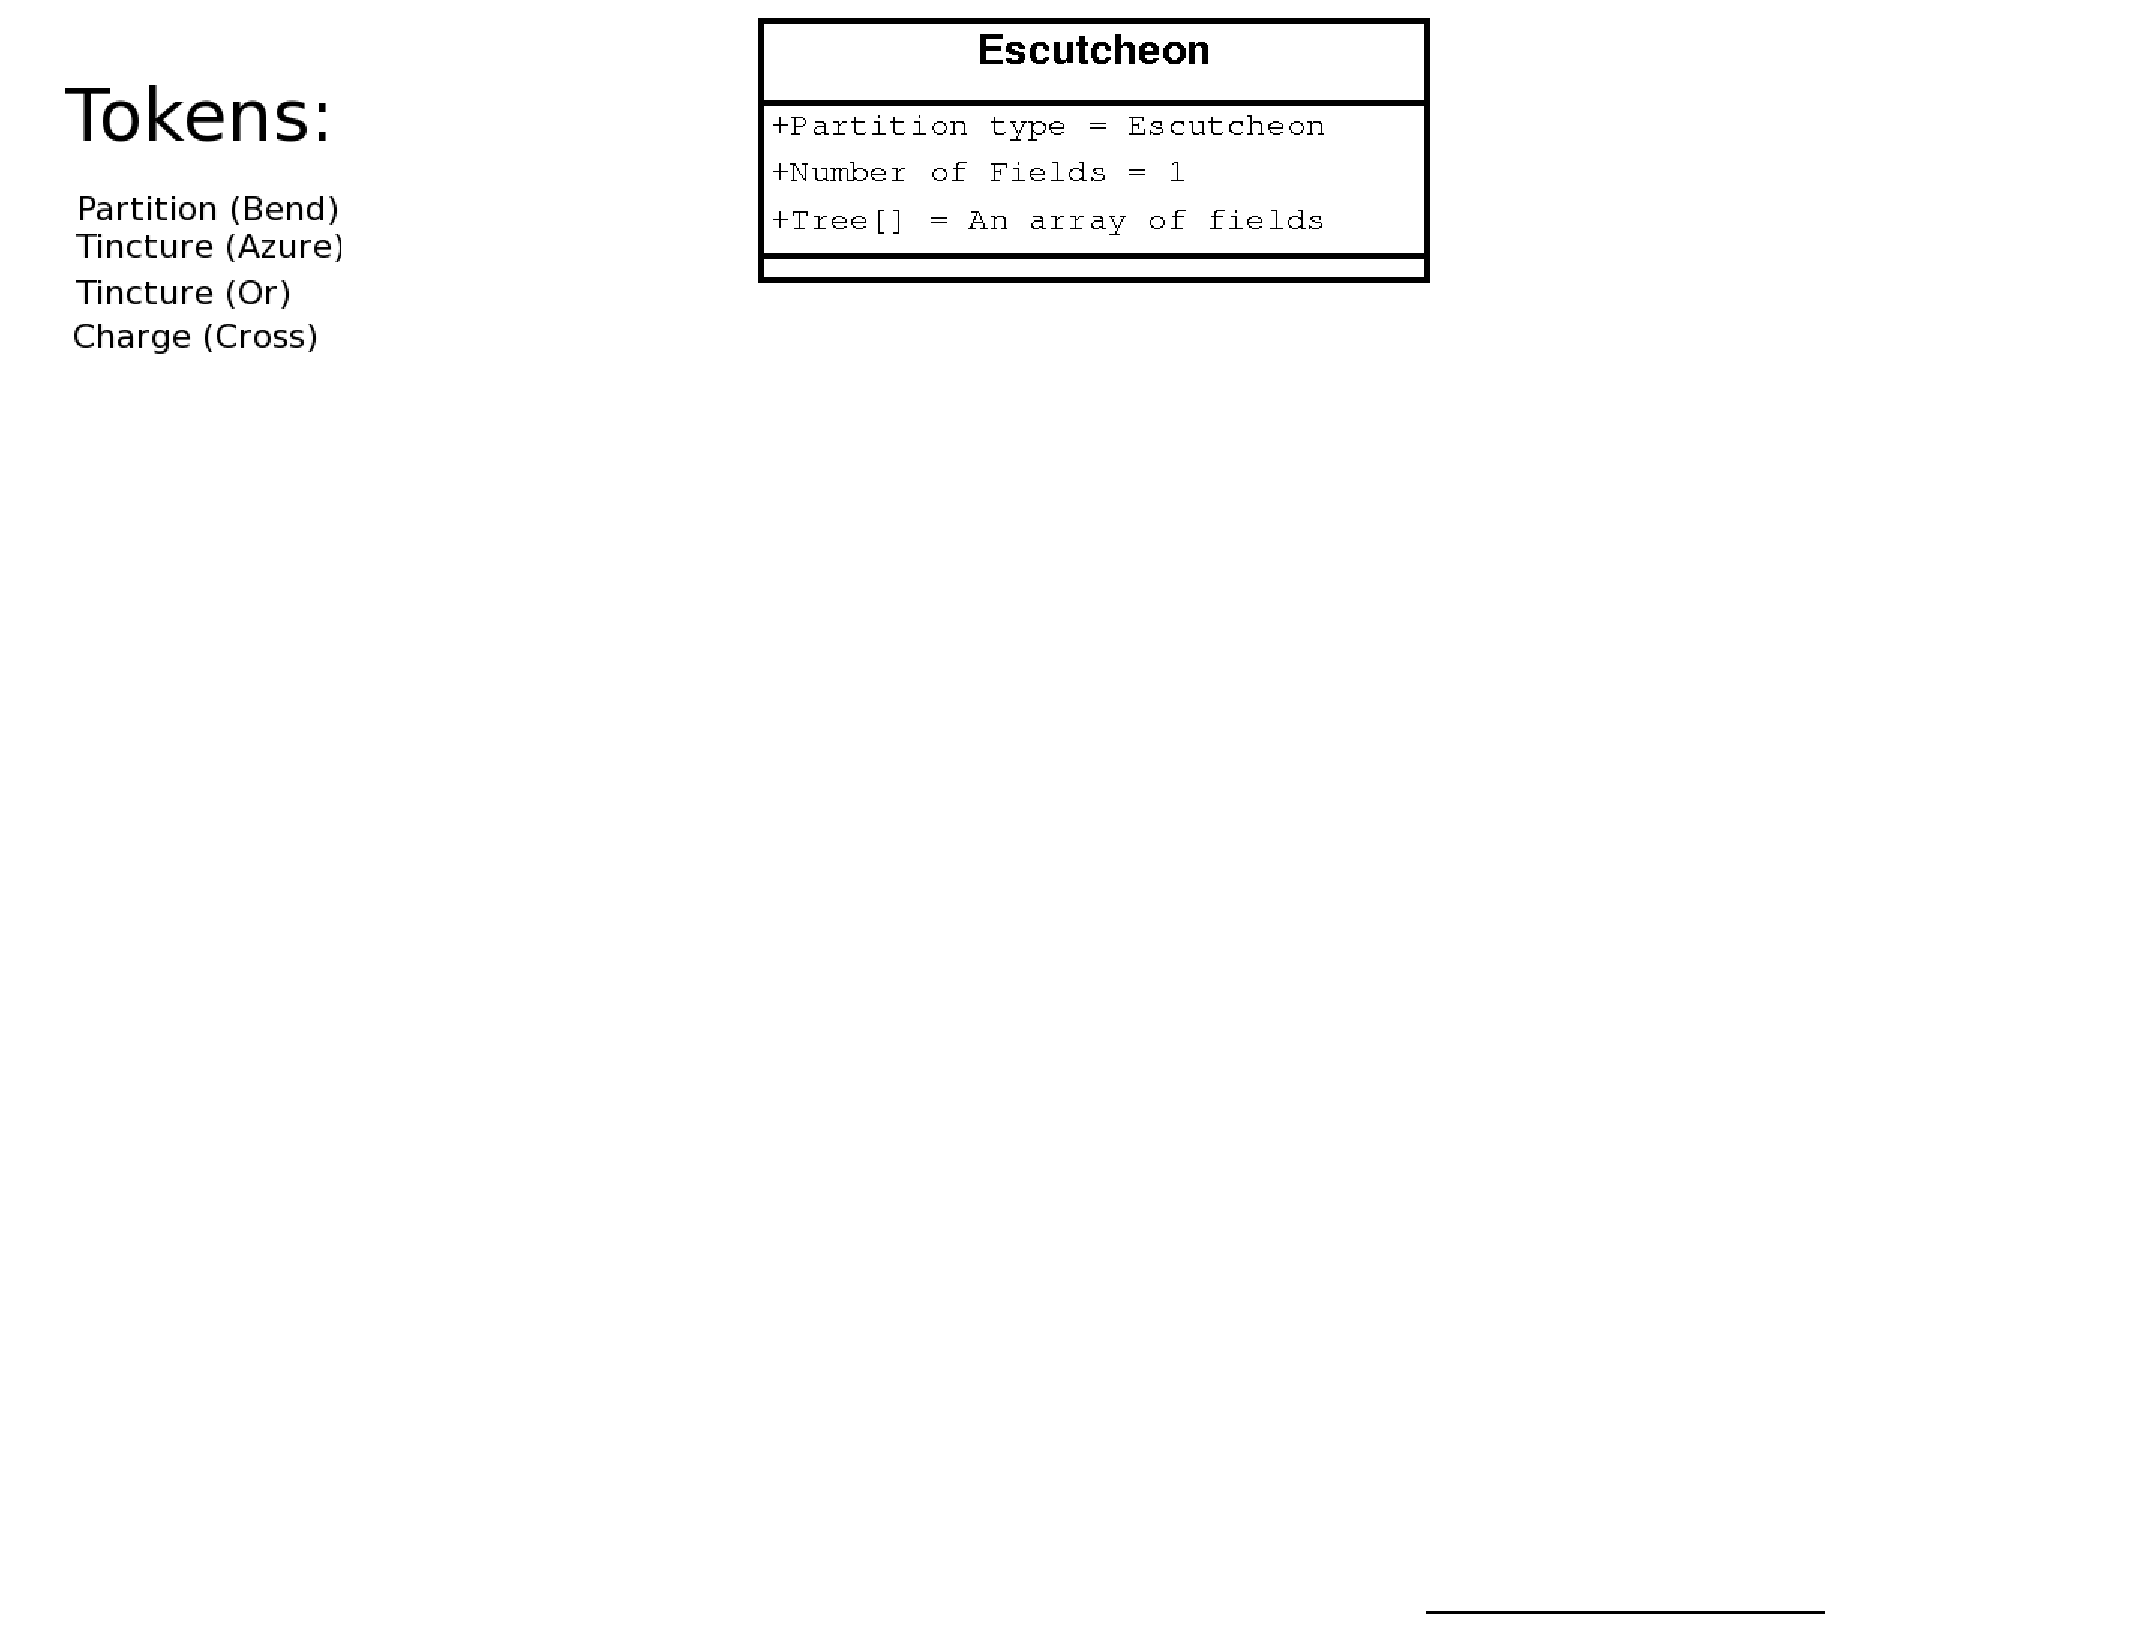
\includegraphics[width=0.8\textwidth]{parsing/images/Parsing5.eps}
  \caption{\emph{"The root of the tree is the implicit Field."}}
  
\end{figure}


\begin{figure}[H]
  \centering
    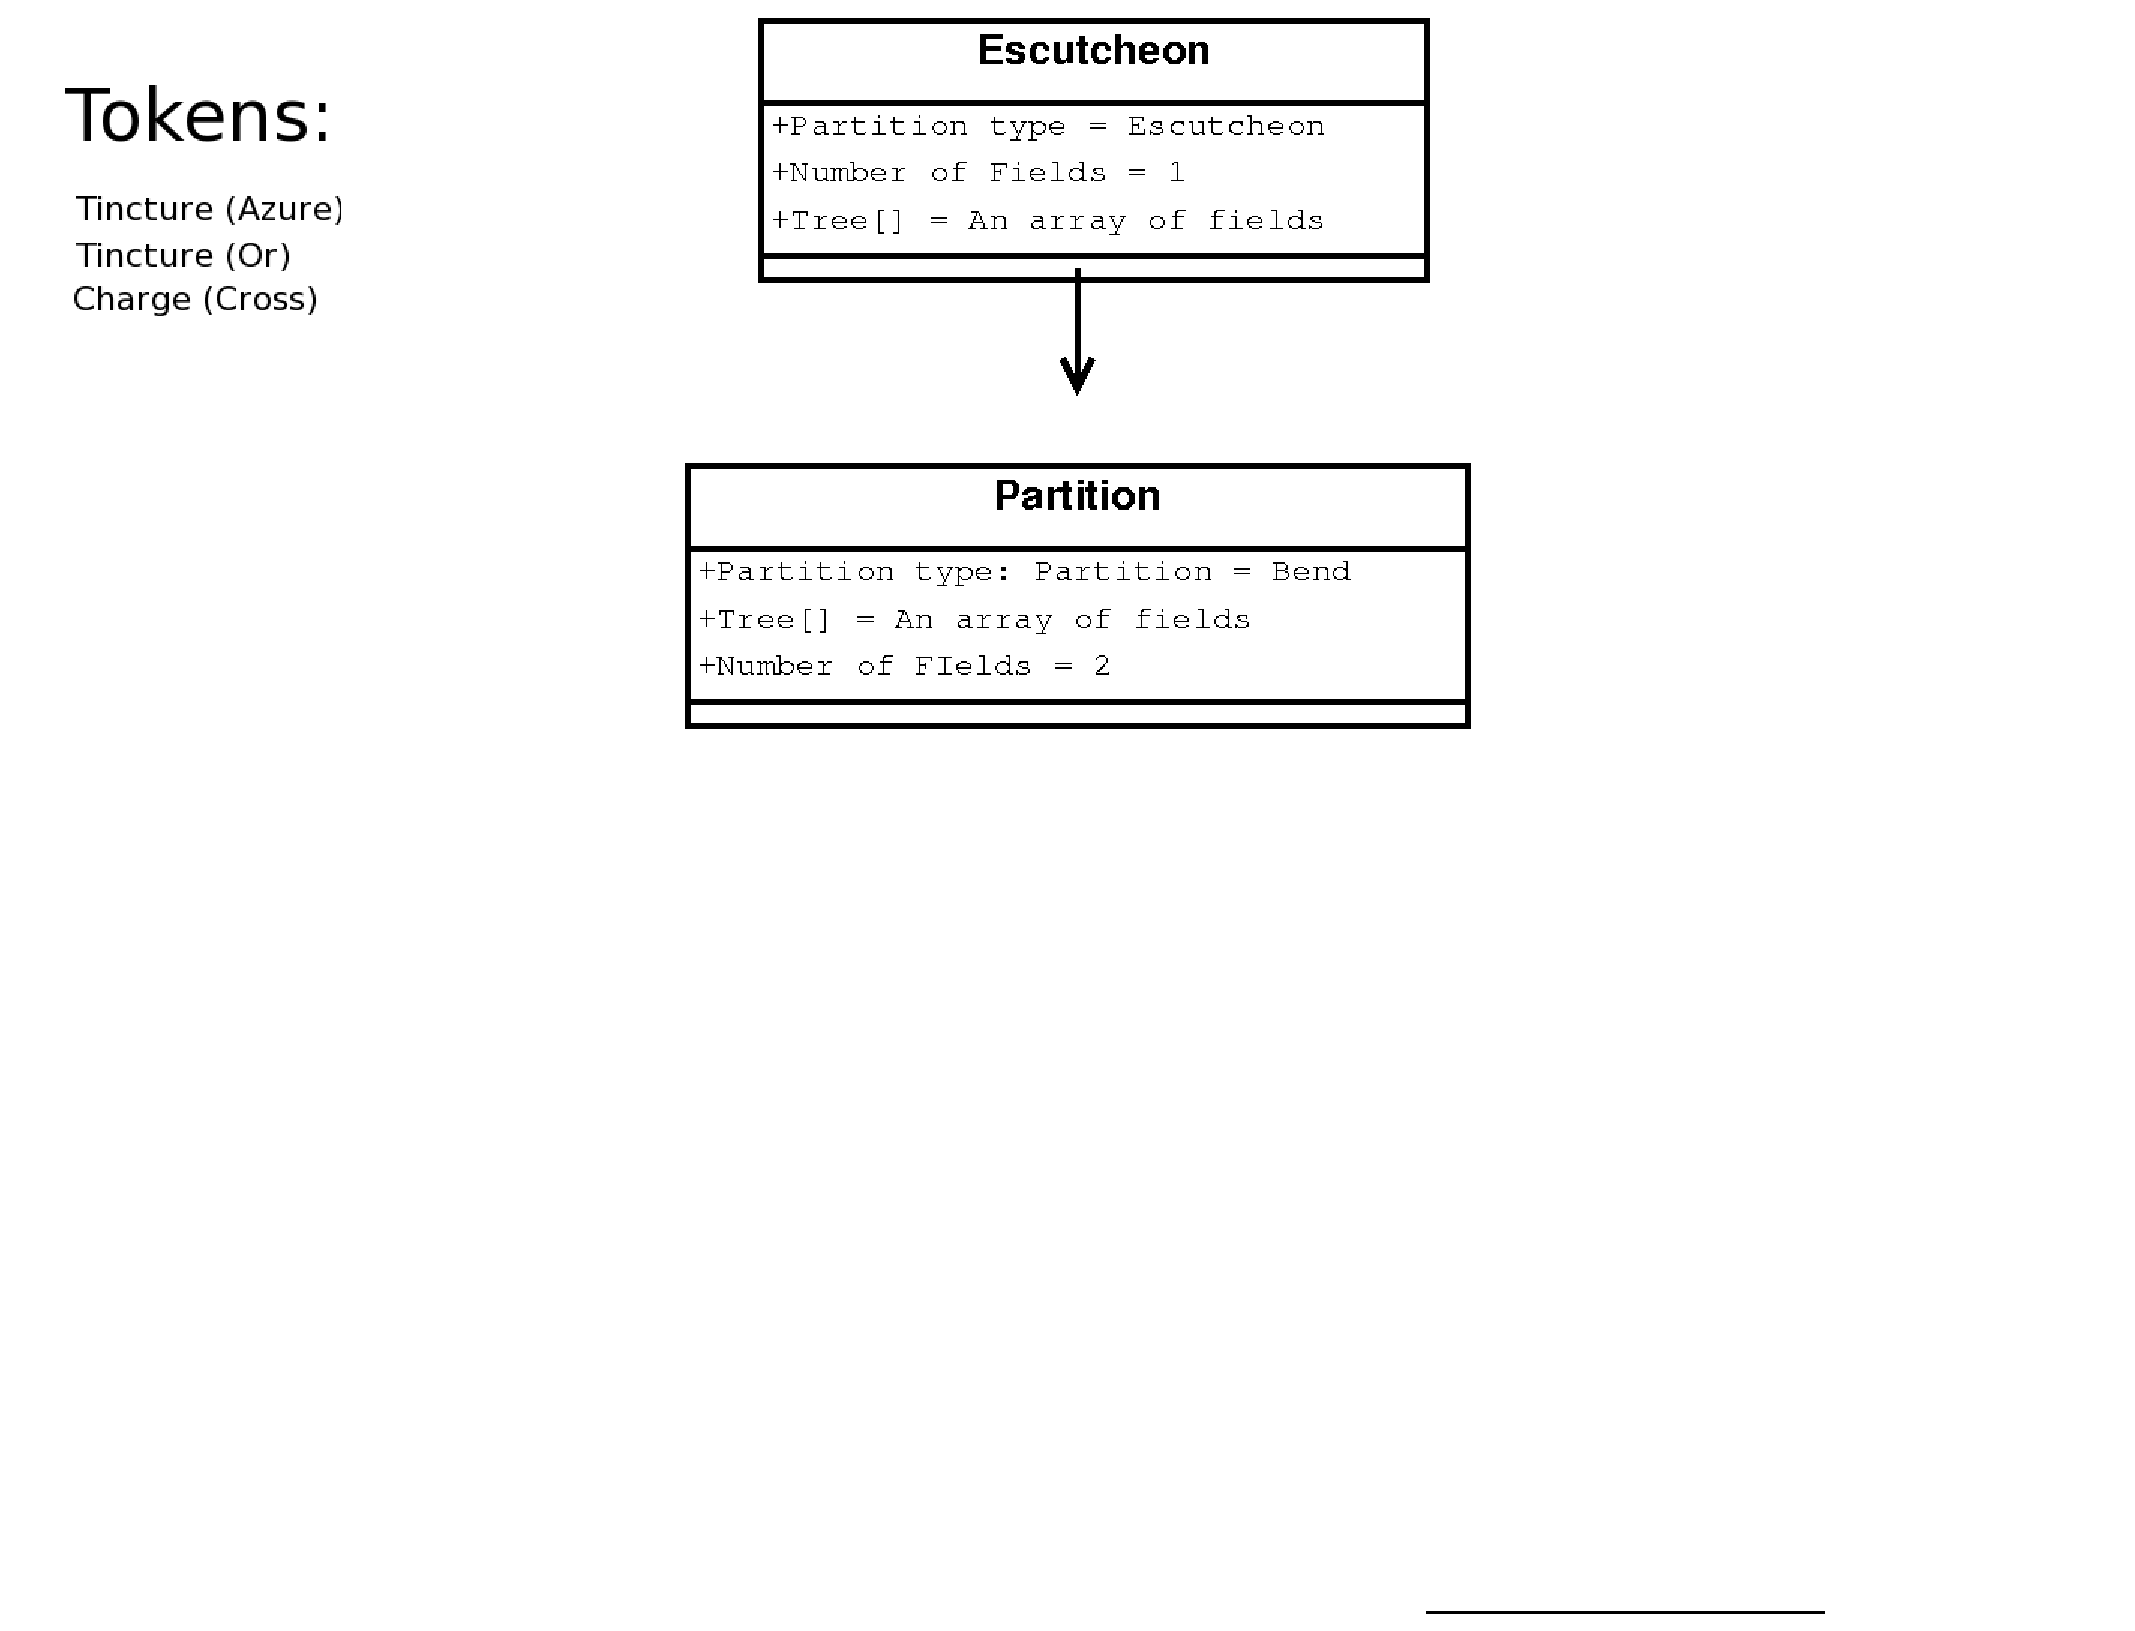
\includegraphics[width=0.8\textwidth]{parsing/images/Parsing4.eps}
  \caption{\emph{"The first token is checked against the grammar then added to the tree array of the initial field."}}
  
\end{figure}


\begin{figure}[H]
  \centering
    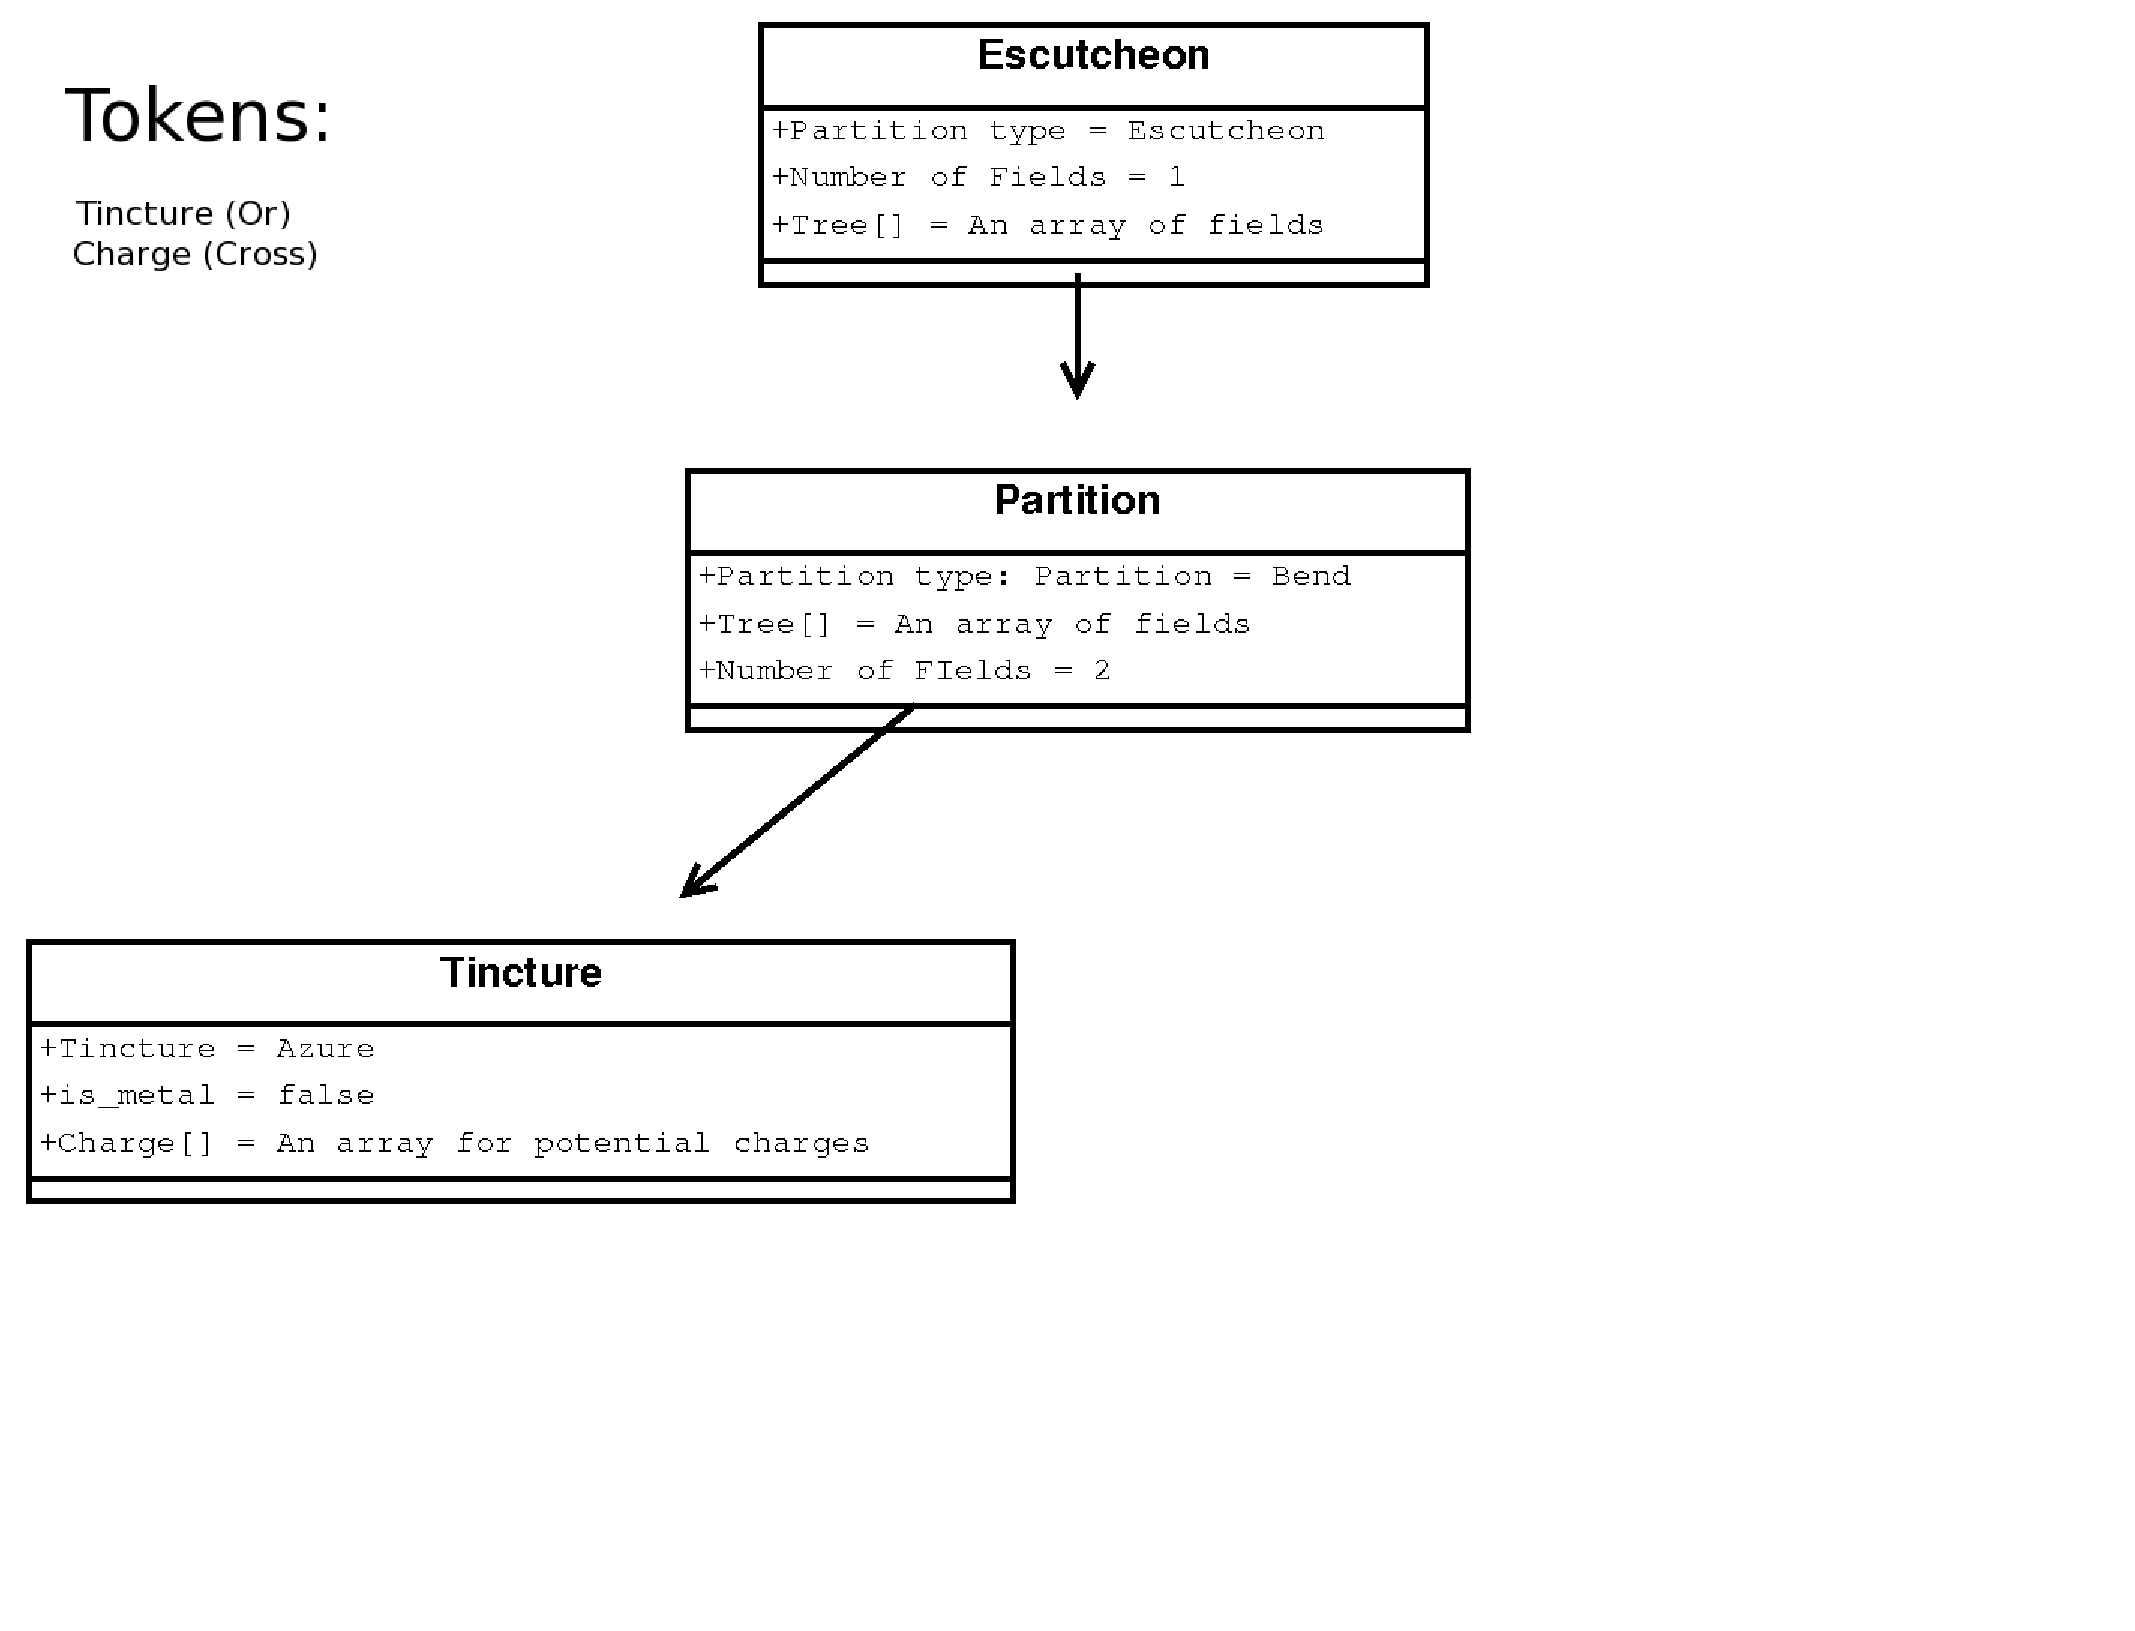
\includegraphics[width=0.8\textwidth]{parsing/images/Parsing3.eps}
  \caption{\emph{"The next token is a Tincture so the first element of the Bend's tree array is assigned to this Tincture"}}
  
\end{figure}

\begin{figure}[H]
  \centering
    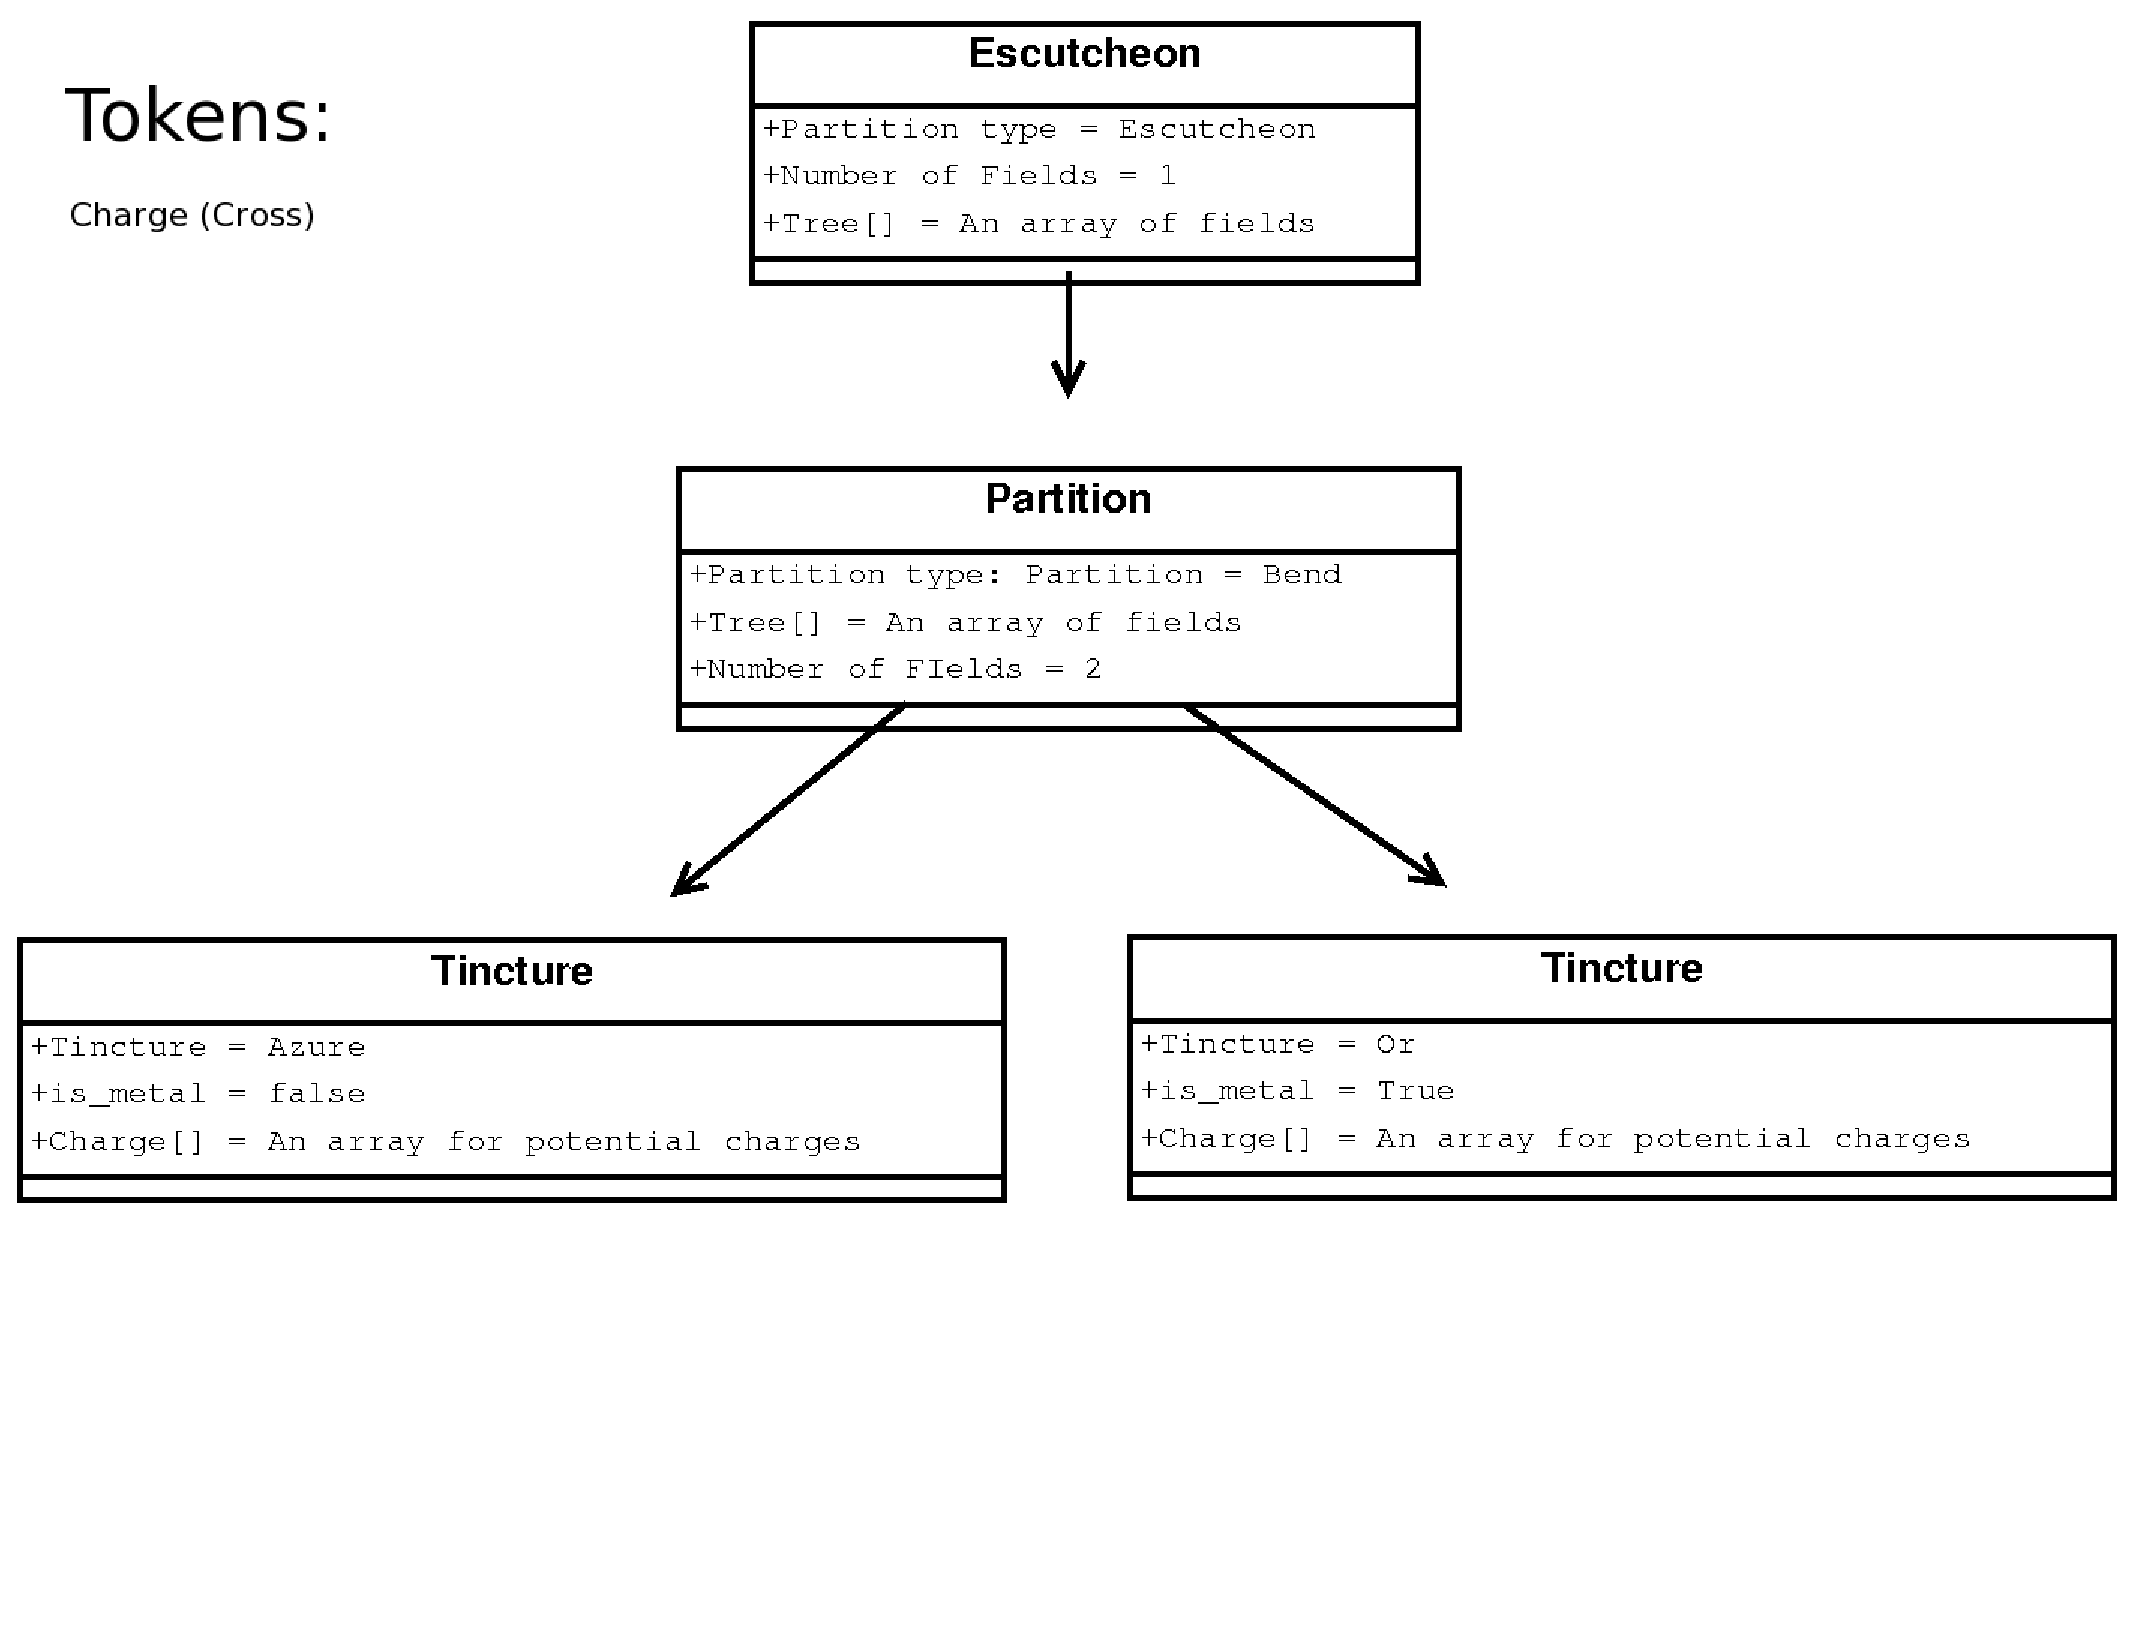
\includegraphics[width=0.8\textwidth]{parsing/images/Parsing2.eps}
  \caption{\emph{"The next token is another Tincture so the second element in the Bend's tree array is assigned to this Tincture."}}
  
\end{figure}

\begin{figure}[H]
  \centering
    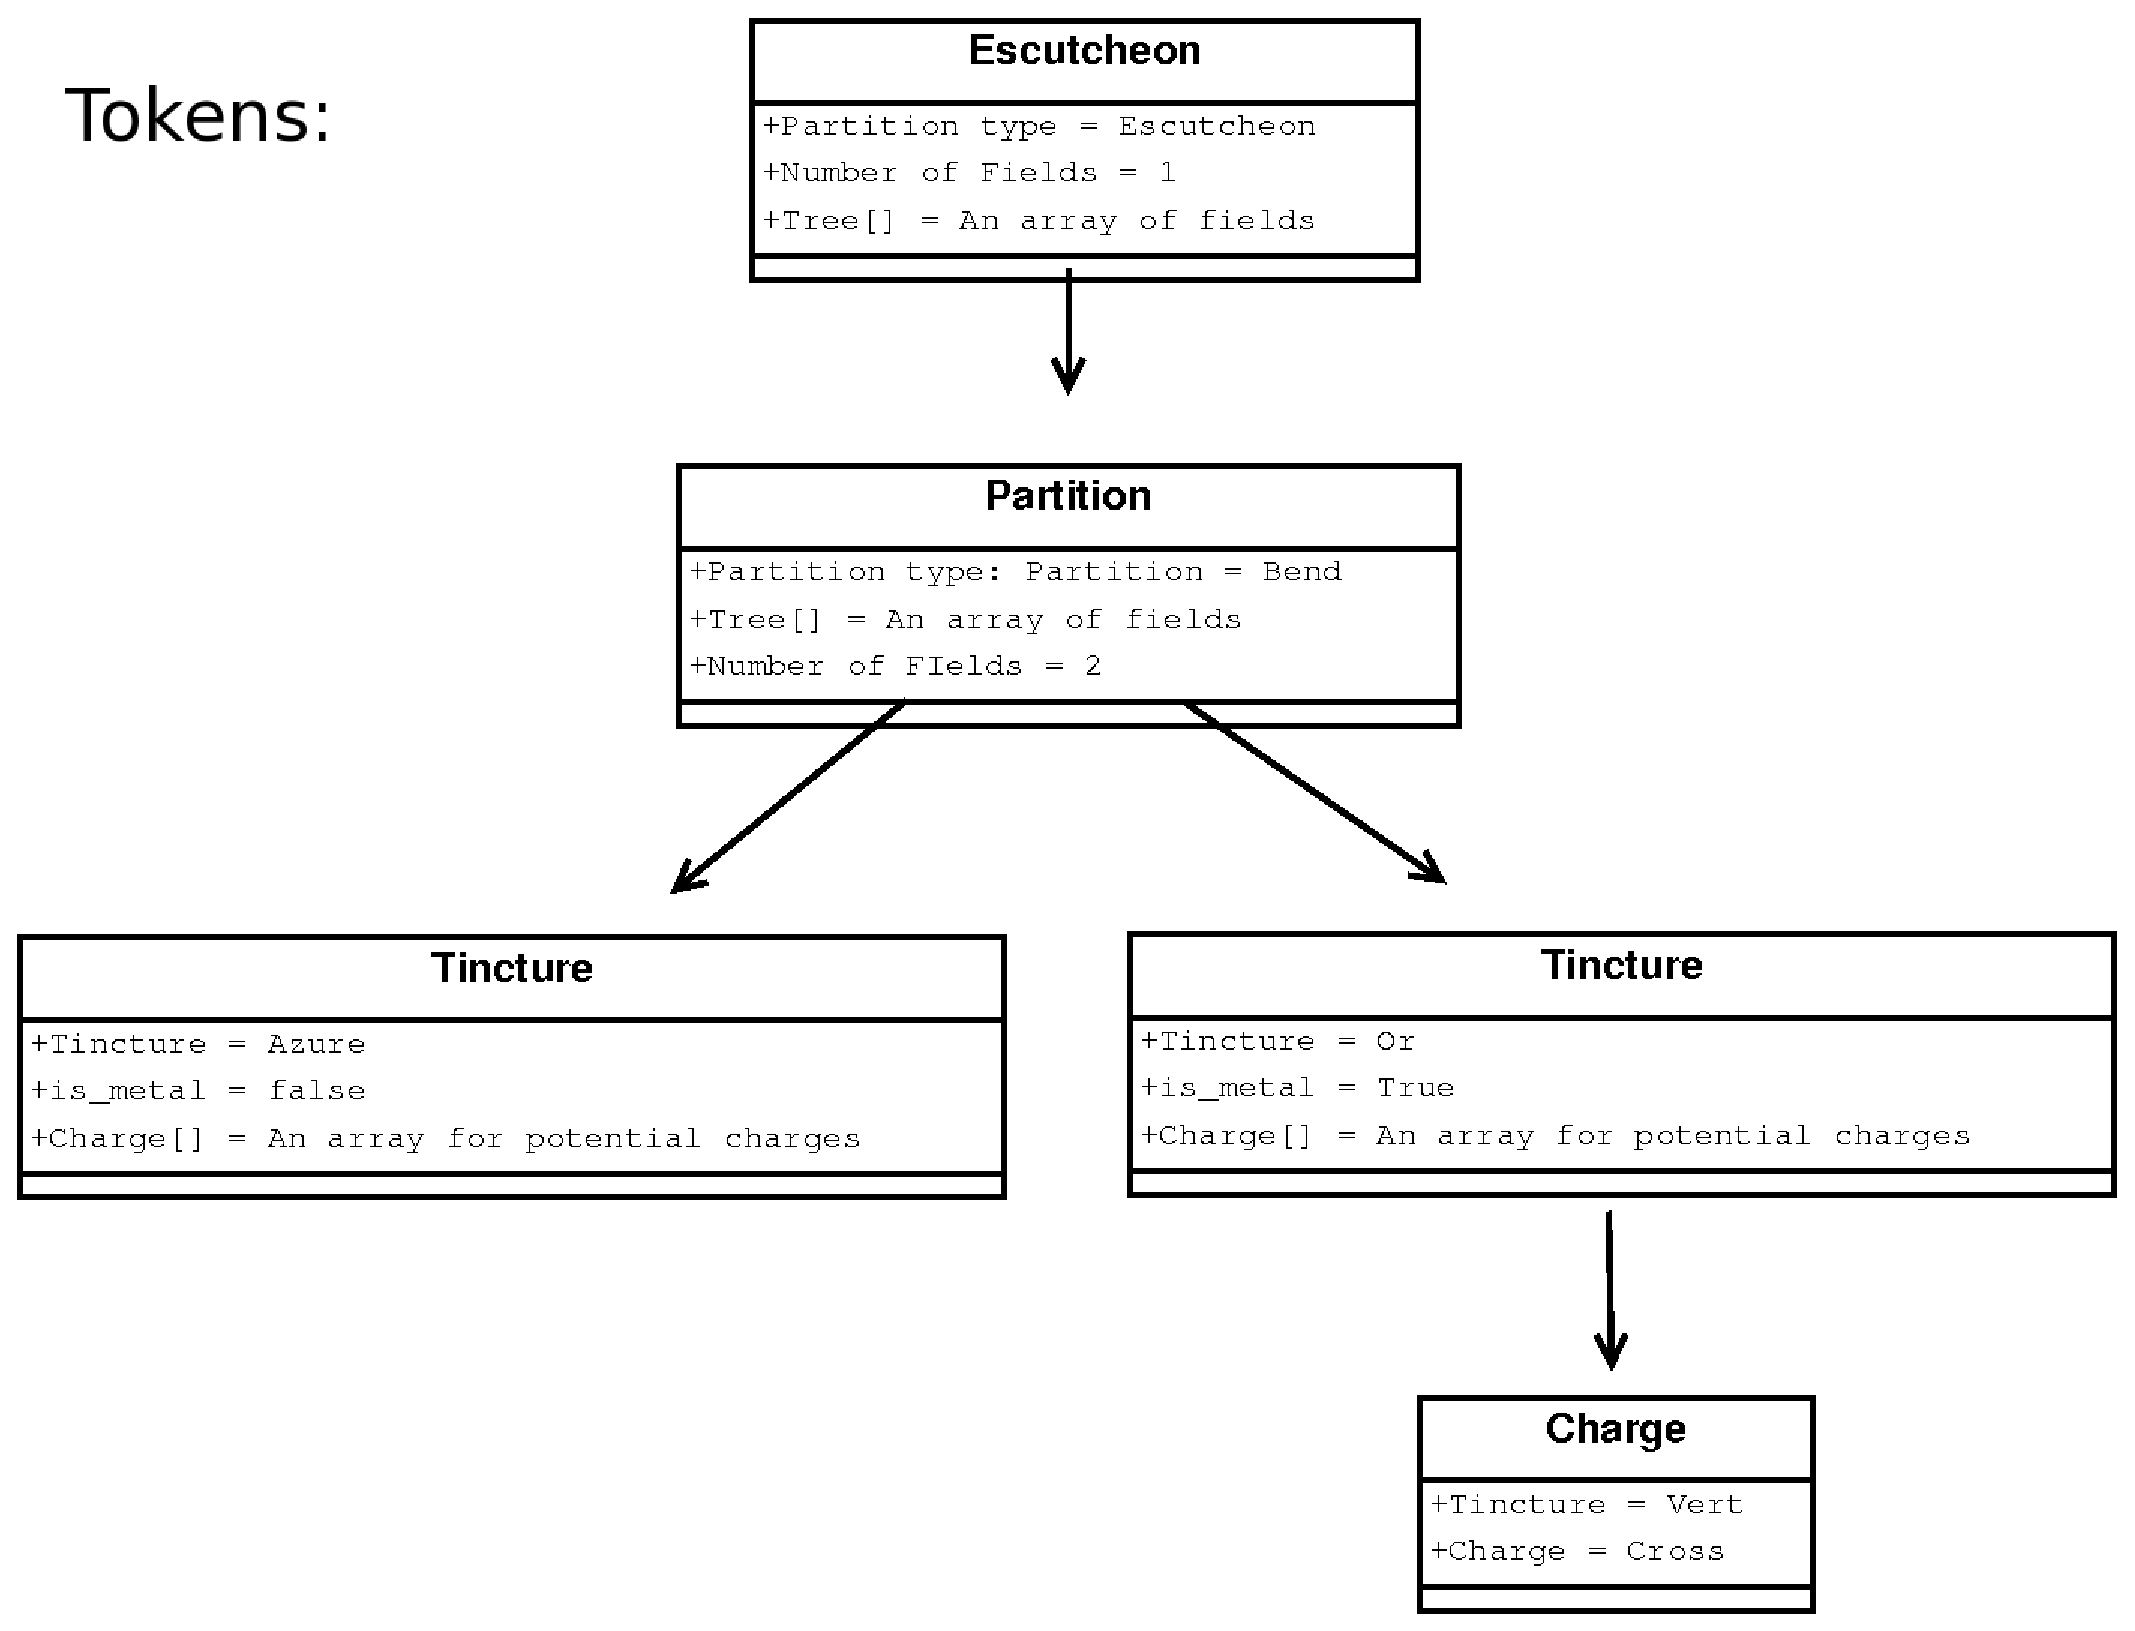
\includegraphics[width=0.8\textwidth]{parsing/images/Parsing1.eps}
  \caption{\emph{"The final token is a Charge as the last token was a Tincture this is a valid token.  The Charge is assigned to the first element of the Or's charge array. As there are no more tokens and no more empty fields this is a valid Blazon sentence and has finished being Parsed."}}
  
\end{figure}

\section{Error Reporting}

If an errors is detected whilst building the Parse tree the Blazon sentence is invalid.  However the end user would benefit greatly if the application could evaluate further as to why the input was erroneous.  Depending upon where in the parse function the error is detected will change what potential errors could have occurred.  The more error reporting that the parser performs the easier it is for the user to correct their mistake. 

The obvious error to address is that of an incomplete Blazon sentence.  If there are no more tokens but the tree has empty nodes in it then the Blazon sentence is invalid because at least one field has yet to be tinctured.  If the inverse is true and there is no space in the tree for the next Token then too many fields have been defined.

The rule of tincture is also enforceable during parsing by checking the parent node's Tincture type against the potential Charge's Tincture.   It is also possible to check that a charge is not placed upon an empty field. 

The most appropriate way to deliver feedback to the user regarding an error is in such a way that they must give it attention.  The application utilises JavaScript alerts for error reporting as the user must acknowledge them before continuing as they are modal, they hold the focus of the browser until acknowledged. 


\section{A Parsing Algorithm}

Pseudo code for implementation of the parsing function used in the web application is given below, in Figure \ref{fig:parse}.  As the implementation was written in JavaScript arrays are objects and upon removing the first element in an array the index of reaming elements are all decremented by one implicitly. 

\begin{figure}[H]
\begin{algorithmic}[1]

\STATE{A recursive function that builds a parse tree from a series of Tokens As input arguments it takes a reference to an array of Tokens provided by Lexical Analysis and the Current node in the Tree, initially the Root node.}

\STATE $Tokens$
\STATE $Current Node$

\WHILE{While there are still empty cells in the current node's tree array}

  \IF{$ Tokens $ is empty}
    \STATE return false
    \COMMENT{as the tree is still being evaluated but no tokens remain there are empty sections remaining on the shield and the Blazon sentence is invalid.}

  \ELSIF{$Tokens[0]$ is a Partition}
    \STATE Push $Tokens[0]$ into the next empty cell of  $CurrentNode$'s tree array
    \STATE Remove the element at $Tokens[0]$ as it has now been parsed
    \STATE Recur passing the $Token$ just placed in  $CurrentNode$'s tree array as the new $CurrentNode$ and a reference to $Tokens$

  \ELSIF{$Tokens[0]$ is a Tincture}
    \STATE Remove the current element at $Tokens[0]$ and place it into the next empty cell in the $Current Nodes$'s tree array. \\
    \COMMENT{Charges can only be placed immediately after a Tincture so can only be valid tokens if found in this control sequence}
    \WHILE{$Tokens[0]$ is a Charge}
      \IF{The Tincture of $Tokens[0]$ is a metal \&\&  The Tincture found was a metal}
        \STATE Rule of Tincture broken
        \STATE return false  
      \ELSIF{The Tincture of $Tokens[0]$ is a colour \&\&  The Tincture found was a colour}
        \STATE Rule of Tincture broken
        \STATE return false  
      \ELSE
        \STATE Remove this Charge from $Tokens[0]$ and add it to the Tincture's Charge Array
      \ENDIF
    \ENDWHILE

  \COMMENT{$Tokens[0]$ is a Charge}
  \ELSE
    \STATE Charges can only be placed immediately after a Tincture which is handled in the above control sequence.    
    \STATE return false  

  \ENDIF
  \STATE return true

\ENDWHILE

\end{algorithmic}
\caption{Pseudo code for Parsing Blazon.}
\label{fig:parse}
\end{figure}






